\documentclass[11pt]{article}
\usepackage[margin=1in]{geometry}
\usepackage[T1]{fontenc}
\usepackage{lmodern}
\usepackage{microtype}
\usepackage{amsmath,amssymb}
\usepackage{booktabs}
\usepackage{array}
\usepackage{enumitem}
\usepackage[font=small]{caption}
\usepackage{pgfplots}
\pgfplotsset{compat=1.18}
\usepackage[hidelinks]{hyperref}
\usepackage{xurl}

\setlist{itemsep=2pt,topsep=4pt}
\newcommand{\code}[1]{\texttt{#1}}
\newcolumntype{L}[1]{>{\raggedright\arraybackslash}p{#1}}
\setlength{\emergencystretch}{3em}
\setcounter{topnumber}{3}
\setcounter{totalnumber}{5}
\renewcommand{\topfraction}{0.9}
\renewcommand{\bottomfraction}{0.6}
\renewcommand{\textfraction}{0.1}
\renewcommand{\floatpagefraction}{0.8}
\setlength{\textfloatsep}{10pt plus 2pt minus 4pt}
\setlength{\floatsep}{8pt plus 2pt minus 2pt}
\setlength{\intextsep}{8pt plus 2pt minus 2pt}
\captionsetup{skip=4pt}

\title{Can Several Minimal Findings Reveal a Hidden Attribute?\\[4pt]
\large An Exactly Solvable Pilot on Linked, Coarsened and Task-Output Releases, with a Release-Audit Toolkit}
\author{Anish Prashun\\ \small Independent researcher}
\date{Independent technical report \quad Version 1.0 \quad November 2026}

\begin{document}
\maketitle

\begin{abstract}
Multi-stage workflows, including AI-assisted ones, often pass small sets of structured findings between stages instead of raw records. We ask how much they reveal about an attribute that none of them states, in a synthetic testbed where every ceiling is computed exactly. A fictional household workflow releases intake (A) and follow-up (B) findings while a three-level reserve band stays hidden. On the same 3,000 test households we compare A, B, both releases linked (C), a declared coarsening of C (D) and the nine report-checklist answers alone (E), using attackers trained on 6,000 labels, exact Bayes and information references, and a deterministic utility measure. The directions of the main effects follow from the construction; their sizes are the result. Linking raised naive-Bayes accuracy by 0.081 over A and 0.068 over B (exact ceilings 0.517, 0.527 and 0.604; baseline 0.400), and one cross-release pair ruled out a band for 5.75\% of households. The coarsening changed accuracy by $-0.018$ [$-0.031$, $-0.006$] on the pre-specified seed, but met this confirmatory criterion in only 3 of 6 seed runs; the power analysis had used the wrong reference gap. The coarsening kept 80.5\% of action items and still leaked more than either single release. The checklist answers kept every action item and still leaked (ceiling 0.565); whether they leak less than a coarsening depends on the checklist. A standard-library toolkit computes these quantities, a per-field information budget and a leakage-utility frontier from a declarative specification. This extends classic composition results; no language model is involved.
\end{abstract}

\section{Introduction}

Workflows that handle personal data are often split into stages, and a common minimisation practice is for each stage to pass downstream a few structured findings rather than the raw record. In an AI-assisted workflow, an intake step may emit a handful of categorical findings, a follow-up step a few more, and a later step composes a report from them. Each set can look harmless. The question is what several of them reveal together about an attribute that none of them states, and what a designer can do about it without breaking the downstream task.

The question is old: composition attacks, sequential releases and the utility cost of generalisation are established (Section~\ref{sec:related}). This report is a focused extension and illustration of those results, not a discovery. It applies the classic comparison of single, linked and generalised releases, plus one alternative that the classic composition papers do not compare, releasing only the task's outputs, to structured findings passed between workflow stages. The AI-workflow setting is motivation only: no language model produces, transforms or attacks anything here.

What the study adds is a testbed in which the answers are computed exactly: the Bayes-optimal accuracy of every view, its mutual information with the hidden attribute, and the accuracy of naive Bayes with unlimited training data come from enumerating a small, fully specified generator. That separates what follows from the construction from what is measured. By construction, the directions of the linking hypothesis (H1) and of the coarsening loss (H2a) hold at the Bayes ceiling, because adding a release cannot lower it and the coarsened view and the task outputs are functions of the linked view; so do the utility ordering (H2b), the confinement of exclusions to the linked view (S3), the absence of unsupported defaults where the strict renderer never abstains (S6), E's full utility, and ``E leaks no more than C''. What is measured is the size of each effect under a documented generator, how close learned attackers with finite labels come to the exact references, and how fragile a pre-specified test is.

\paragraph{Contributions.}
\begin{enumerate}
  \item An exactly solvable testbed in which every ceiling is computed rather than estimated, logical exclusion is reported apart from statistical inference, and utility is a deterministic task checklist split into supported and unsupported answers.
  \item Effect sizes under a documented generator, from a protocol frozen before test scoring (self-attested), including a confirmatory result (H2a) that holds on the pre-specified seed but meets its criterion in only 3 of 6 seed runs.
  \item An exploratory comparison showing that task outputs dominate the linked fine release but are not ordered against a coarsening in general.
  \item \code{release\_audit}, a standard-library toolkit that computes the same exact quantities, a per-field information budget and a release-design frontier for a user's own specification.
\end{enumerate}

\section{Related work}
\label{sec:related}

\paragraph{Composition and sequential release.} Ganta et al.~\cite{ganta2008composition} showed that independently anonymised releases about overlapping populations can be combined: their intersection attack intersects the candidate sensitive values left by each release and breaches $k$-anonymity and its variants, whereas definitions in the style of differential privacy provably resist composition attacks. Wang and Fung~\cite{wang2006sequential} showed that joining a new release with an earlier one about the same people can enable sensitive inference, and generalised the new release so that the join becomes lossy while each release keeps its own information requirement; Xiao and Tao~\cite{xiao2007minvariance} showed similar failures under repeated publication. Our view C is the joined release. Our exclusions are not an instance of the intersection attack, which intersects the sensitive values each release leaves possible: neither of our releases rules out a band on its own, and the exclusion arises only when the two are joined, as in Wang and Fung's observation that the join ``enables inferences across tables''. Unlike Wang and Fung, we assume the linkage is known, so coarsening gets no credit for hiding the join.

\paragraph{Generalisation, information and baselines.} Generalising values into coarser categories is a standard remedy~\cite{samarati2001protecting,sweeney2002generalization}. Brickell and Shmatikov~\cite{brickell2008cost} measured privacy loss as the adversary's gain in learning sensitive attributes and utility as data-mining accuracy on the same records, and concluded that ``even modest privacy gains require almost complete destruction of the data-mining utility''. Kifer~\cite{kifer2009definetti} attacked partition-based sanitisation with a naive Bayes classifier, our main attacker's model family. Query-view security asks whether published views disclose a secret query~\cite{miklau2004formal}, and quantitative information flow bounds the leakage of composed channels, including parallel channels on one secret~\cite{kawamoto2017compositionality}. Attribute inference should be compared with an imputation baseline that has the same distributional knowledge~\cite{jayaraman2022imputation}; we report every leak as a gain over the frequency baseline and call what we measure distributional inference. Our utility is a fixed downstream checklist, which is what makes the task-output alternative (E) definable.

\paragraph{Language-model systems.} Language models infer personal attributes from text~\cite{staab2024beyond,yukhymenko2024synthpai}. Patil et al.~\cite{patil2025sum} studied multi-agent systems in which a hidden attribute emerges only from combining individually innocuous outputs (single-source leakage is zero by construction, and the defences block or refuse); Asif and Amiri~\cite{asif2026information} formalised compositional leakage along sequential agent pipelines with mutual information. Zhou et al.~\cite{zhou2025minimization} searched for the least revealing transformation of a single prompt, including abstraction, that passes a utility check, without studying several releases; ToolPrivacyBench~\cite{hu2026toolprivacybench} counts private facts that reach unauthorised tools, by presence rather than inference; AgentDAM~\cite{zharmagambetov2025agentdam} and AirGapAgent~\cite{bagdasarian2024airgapagent} evaluate or enforce data minimisation for agents. We measure graded gains over single releases and use the checklist as the utility predicate.

\paragraph{Position.} A literature search found no study that runs exactly this comparison on the same held-out individuals with exact Bayes references and a separate deterministic utility measure. The nearest recent work we found treats sequential releases to colluding receivers information-theoretically, with mutual-information leakage, a separate utility and optimised randomised releases~\cite{taylor2026adaptive}; it does not compare coarsened or task-output releases or report Bayes-accuracy ceilings. The search was not exhaustive, and every ingredient is established.

\section{Setting and threat model}
\label{sec:setting}

Each synthetic household has a hidden reserve band: \code{low} (liquid reserve under one month of essential costs), \code{medium} (one to three months) or \code{high} (more than three). Release~1 (intake) has five categorical fields, release~2 (follow-up) has four, and a downstream step fills a nine-item report checklist. The band exists only in the scoring data, there is no free text, and every probability is invented.

\begin{itemize}
  \item \textbf{View and linkage.} The attacker sees only what a downstream system would receive in a given condition (Section~\ref{sec:conditions}). In the linked conditions it is told that both releases belong to the same household; how hard linkage is in practice is out of scope. In the study's own data files the release-1 and release-2 views carry the same opaque household identifier: a stable key across stages is exactly the linkage assumed.
  \item \textbf{Knowledge.} 6,000 labelled training households from the same generator, in the same representation: a strong, upper-bound attacker for its model family (Section~\ref{sec:controls} adds weaker ones). It never sees the band (except in a labelled positive control), seeds, label-correlated file order or any other condition's representation; identifiers are opaque HMAC values and test rows are shuffled.
  \item \textbf{Isolation.} Each attacker runs as a separate \code{python3 -I} process in a fresh, empty directory, with an otherwise empty environment and its input on standard input only: process-level isolation, not an operating-system sandbox.
\end{itemize}

Leakage is a gain over a frequency baseline that predicts the most common band. \emph{Statistical inference} shifts the attacker's posterior; \emph{logical deduction} occurs when a released value has probability zero under some band, which it then \emph{excludes} (it \emph{determines} the band if only one remains).

\section{Generator and conditions}
\label{sec:conditions}

\begin{table}[htbp]
\centering\footnotesize
\caption{Generator of the main scenario ($\lambda = 1$). Cells give $P(\text{value} \mid \text{band})$ in the listed value order. The resolution is \code{not\_applicable} exactly when there is no event. The 0.00 for a low-band household settling a major expense in full is the one hard zero. Every probability is invented.}
\label{tab:generator}
\setlength{\tabcolsep}{3pt}
\begin{tabular}{@{}L{3.0cm}L{3.75cm}L{2.95cm}L{2.95cm}L{2.95cm}@{}}
\toprule
Field & Values, in order & \code{low} & \code{medium} & \code{high} \\
\midrule
Prevalence $\pi$ & & 0.40 & 0.35 & 0.25 \\
\code{r1.income\_pattern} & $P(\code{irregular})$ & 0.50 & 0.35 & 0.25 \\
\code{r1.essential\_share} & \code{under\_50}, \code{50\_70}, \code{over\_70} & 0.15, 0.40, 0.45 & 0.30, 0.45, 0.25 & 0.50, 0.35, 0.15 \\
\code{r1.event\_code} & \code{none}, \code{vehicle\_minor}, \ldots, \code{home\_major} & \multicolumn{3}{L{9.0cm}}{Independent of the band: $P(\text{event}) = 0.50$, type uniform, $P(\code{major} \mid \text{event}) = 0.40$} \\
\code{r1.payment\_flag} & \code{none}, \code{late\_utility}, \code{overdraft\_fee}, \code{both} & 0.45, 0.20, 0.20, 0.15 & 0.65, 0.15, 0.12, 0.08 & 0.85, 0.07, 0.06, 0.02 \\
\code{r1.contact\_channel} & \code{email}, \code{phone}, \code{post} & \multicolumn{3}{L{9.0cm}}{Independent of the band: 0.60, 0.30, 0.10} \\
\code{r2.resolution}, minor event & \code{settled\_in\_full}, \code{instalment\_plan}, \code{outstanding} & 0.60, 0.25, 0.15 & 0.75, 0.18, 0.07 & 0.85, 0.12, 0.03 \\
\code{r2.resolution}, major event & same & 0.00, 0.45, 0.55 & 0.25, 0.55, 0.20 & 0.80, 0.17, 0.03 \\
\code{r2.payment\_flag} & as \code{r1.payment\_flag} & 0.50, 0.18, 0.18, 0.14 & 0.70, 0.13, 0.10, 0.07 & 0.88, 0.06, 0.05, 0.01 \\
\code{r2.goal} & \code{none}, \code{build\_buffer}, \code{reduce\_debt}, \code{major\_purchase} & 0.25, 0.35, 0.30, 0.10 & 0.30, 0.25, 0.25, 0.20 & 0.35, 0.10, 0.15, 0.40 \\
\code{r2.document\_status} & \code{complete}, \code{missing\_id}, \code{missing\_income\_proof} & \multicolumn{3}{L{9.0cm}}{Independent of the band: 0.70, 0.15, 0.15} \\
\bottomrule
\end{tabular}
\end{table}

Table~\ref{tab:generator} gives the generator. Income pattern, essential-cost share, both payment flags (conditionally independent given the band) and the savings goal carry moderate additive band information. The event's size (release~1) and its resolution (release~2) interact: size alone carries no band information, resolution alone some, and a major expense settled in full is strong evidence of a high reserve. One hard constraint is planted: a low-reserve household cannot settle a major expense in full, so the pair (\code{major}, \code{settled\_in\_full}) excludes \code{low}, and only the linked fine view shows the pair. Contact channel, document status and the event's occurrence and type carry no band information but are needed for the report. Raw households take 65,664 distinct value combinations with positive probability.

\paragraph{Scenarios.} Every scenario has its own 10,000 households, split by household into 6,000 training, 1,000 development and 3,000 test households. Sensitivity scenarios mix each conditional distribution toward its marginal, $P_\lambda(f \mid b) = (1 - \lambda) M(f) + \lambda P(f \mid b)$ with $M(f) = \sum_b \pi(b) P(f \mid b)$, at $\lambda = 0$ (\code{independence}, a control), 0.25, 0.50 and 0.75; two more keep $\lambda = 1$ and make the prevalence uniform (\code{prev\_balanced}) or 0.70, 0.20, 0.10 (\code{prev\_skewed}). Exclusions can occur only when $\lambda = 1$. A positive control plants the band as a field in both releases. The main scenario is regenerated from five further master seeds; with the primary run these give six seed runs, each with its own households, split and training.

\paragraph{Conditions.} Every condition is computed for the same test households: \textbf{A}, release 1 only; \textbf{B}, release 2 only; \textbf{C}, both releases linked as one record; \textbf{D}, C after a declared coarsening; and \textbf{E}, the nine checklist answers only (Table~\ref{tab:checklist}), the minimal output the report needs, pre-specified as a secondary condition. The coarsening renames each field it changes so that granularity is explicit, and drops no field: \code{under\_50} and \code{50\_70} shares become \code{up\_to\_70}; the event code loses its size (\code{medical\_major} becomes \code{medical}); each payment flag becomes \code{none} or \code{any}; and \code{settled\_in\_full} and \code{instalment\_plan} become \code{arranged}. Income pattern, contact channel, goal and document status pass through unchanged.

\begin{table}[htbp]
\centering\footnotesize
\caption{The report checklist. Correct answers come from the full raw record. The last column is E's exact input for the worked example of Table~\ref{tab:example}.}
\label{tab:checklist}
\begin{tabular}{@{}llL{6.3cm}l@{}}
\toprule
Item & Values & Correct answer & Example \\
\midrule
\code{budget\_session} & yes, no & yes iff either payment flag is not \code{none} & yes \\
\code{overdraft\_guidance} & yes, no & yes iff either flag is \code{overdraft\_fee} or \code{both} & yes \\
\code{essential\_cost\_review} & yes, no & yes iff the share is \code{over\_70} & no \\
\code{expense\_referral} & \code{none} or a type & the event type iff an event occurred and its resolution is \code{instalment\_plan} or \code{outstanding} & \code{medical} \\
\code{hardship\_review} & yes, no & yes iff a major event is \code{outstanding} & no \\
\code{plan\_monitoring} & yes, no & yes iff the resolution is \code{instalment\_plan} & yes \\
\code{goal\_module} & \code{none} or a goal & the goal & \code{build\_buffer} \\
\code{documents\_request} & \code{none}, \code{id}, \code{income\_proof} & from the document status & \code{income\_proof} \\
\code{contact\_channel} & \code{email}, \code{phone}, \code{post} & the channel & \code{phone} \\
\bottomrule
\end{tabular}
\end{table}

\begin{table}[htbp]
\centering\footnotesize
\caption{Worked example: hand-checked household H1 of the protocol (true band \code{medium}). Each condition receives exactly these key-value pairs as one JSON line: A the release-1 rows, B the release-2 rows, C all nine, D the right-hand columns, and E the answers in Table~\ref{tab:checklist}. The last row counts the strict renderer's correct items out of nine.}
\label{tab:example}
\begin{tabular}{@{}llll@{}}
\toprule
Fine field (A or B, and C) & Value & Field in D & Value in D \\
\midrule
\code{r1.income\_pattern} & \code{regular} & \code{r1.income\_pattern} & \code{regular} \\
\code{r1.essential\_share} & \code{50\_70} & \code{r1.essential\_share\_coarse} & \code{up\_to\_70} \\
\code{r1.event\_code} & \code{medical\_major} & \code{r1.event\_type} & \code{medical} \\
\code{r1.payment\_flag} & \code{overdraft\_fee} & \code{r1.payment\_difficulty} & \code{any} \\
\code{r1.contact\_channel} & \code{phone} & \code{r1.contact\_channel} & \code{phone} \\
\code{r2.resolution} & \code{instalment\_plan} & \code{r2.resolution\_coarse} & \code{arranged} \\
\code{r2.payment\_flag} & \code{none} & \code{r2.payment\_difficulty} & \code{none} \\
\code{r2.goal} & \code{build\_buffer} & \code{r2.goal} & \code{build\_buffer} \\
\code{r2.document\_status} & \code{missing\_income\_proof} & \code{r2.document\_status} & \code{missing\_income\_proof} \\
\midrule
\multicolumn{4}{@{}l}{Strict renderer, items correct of 9: A 4, B 4, C 9, D 6, E 9} \\
\bottomrule
\end{tabular}
\end{table}

In the worked example (Table~\ref{tab:example}), D's \code{any} hides whether the release-1 flag was an overdraft fee and \code{arranged} hides whether there is an instalment plan, so the report cannot settle overdraft guidance, the referral or plan monitoring. A second hand example shows \code{home\_major} in release~1 and \code{settled\_in\_full} in release~2: neither release excludes anything alone, the linked pair excludes \code{low}, and D cannot, because coarsening removes the size.

\section{Attackers, references, renderers and measures}
\label{sec:method}

\paragraph{Attackers.} All attackers receive the training rows and labels of one view and the test rows of the same view, and none abstains. Arithmetic is exact, and ties break in the order low, medium, high. \code{baseline} predicts the most frequent training band. \code{nb} is categorical naive Bayes over all visible fields, with an add-1 smoothed prior and add-$\alpha$ smoothing ($\alpha = 1$) per field over the values seen in training plus one slot for unseen values. \code{nb\_pair} is \code{nb} with one schema-linked cross-release pair joined into a single feature, (\code{event\_code}, \code{resolution}) in C and (\code{event\_type}, \code{resolution\_coarse}) in D; elsewhere it equals \code{nb}. \code{lookup} predicts from the add-1 smoothed band counts of the full visible tuple when that tuple occurs at least $m = 5$ times in training, and otherwise falls back to \code{nb}.

\paragraph{Exact references.} The \emph{oracle}, a reference rather than an attacker, is the exact Bayes posterior under the true generator, $P(b \mid v) \propto \pi(b) P(v \mid b)$, from enumerating every raw household; scored on the test households it is the ``sample oracle''. The enumeration also gives the population Bayes accuracy $\sum_v \max_b \pi(b) P(v \mid b)$, $I(\text{band}; \text{view})$ and $H(\text{band} \mid \text{view})$ in bits, the mass of view values that exclude a band, and \code{nb\_limit}, the exact accuracy of \code{nb} with unlimited training data (likewise for \code{nb\_pair}). The fields are conditionally independent given the band apart from the size-resolution pair (and a band-independent duplication of ``no event''), so \code{nb\_limit} equals the Bayes ceiling exactly in A, B and D, and \code{nb\_pair}'s limit equals it in C, where its one joined pair is the generator's one interaction (Table~\ref{tab:population}). That learned attackers approach the ceilings is expected by design and says nothing about attackers in general.

\paragraph{Renderers and utility.} The \emph{strict} renderer reads only the supplied view and abstains unless the view entails the answer; for E it reads the answers directly. The \emph{default-filling} renderer emits a default (\code{no}, \code{none}, or \code{email} for the channel) wherever the strict renderer abstains. An \emph{action item} is a (household, item) pair whose correct answer is \code{yes} or not \code{none}; the contact channel always is one. Each output is \emph{supported-correct} (entailed by the view), \emph{unsupported-correct} (a lucky default), \emph{unsupported-wrong}, or an \emph{omission}, and only supported outputs earn action-item credit. This split was added after the review; the original protocol counted lucky defaults as correct.

\paragraph{Measures.} On the test split, per scenario, view and attacker: accuracy (correct out of 3,000), macro recall, and mean log-loss in bits, $-\log_2 p(\text{true band})$ with probabilities clipped below at $10^{-12}$. Intervals are 95\% percentile bootstraps with 2,000 resamples of test households, resampled jointly across views for paired differences. They cover test-sample uncertainty only: each attacker is fitted once per dataset, and the seed runs show training and generator variability. There is no correction for multiple comparisons; only H1a, H1b and H2a are confirmatory.

\section{Pre-specification and validation}
\label{sec:prespec}

\paragraph{Hypotheses.} The confirmatory hypotheses use \code{nb} on the test split of \code{main}. \textbf{H1a:} accuracy C $-$ A $> 0$ and \textbf{H1b:} C $-$ B $> 0$, each with a 95\% interval excluding 0. \textbf{H2a:} D $-$ C $< 0$, with a 95\% interval excluding 0. \textbf{H2b}, strict-renderer action items conveyed D $>$ max(A, B) and D $<$ C, was listed as confirmatory in v1.0 and relabelled descriptive in v1.1, because the generator and the renderer fix its outcome. Controls: in \code{independence} every attacker must be within 0.05 of baseline accuracy; in the positive control \code{nb} must reach at least 0.99 in A--D with 3,000 directly exposed test rows in each; elsewhere there must be no direct exposure.

\paragraph{Sample size, and an error in the power analysis.} Before the freeze, we enumerated the generator and found a C $-$ D gap of only about 3 accuracy points at the Bayes ceiling; with 600 test households the paired 95\% interval would also have had a half-width of about 3 points, so the households per scenario were raised from 3,000 to 10,000 before any data were scored. That analysis contained an error of ours: it sized H2a from the Bayes-optimal gap, but H2a is tested with \code{nb}, which cannot use the size-by-resolution interaction that the coarsening removes (Section~\ref{sec:confirmatory}). It also printed D's ceiling as 0.576, a double rounding of the exact 0.575466; the protocol now reads 0.5755, and no output used the printed value.

\paragraph{Freeze history.} The freeze records SHA-256 hashes of the protocol, fixtures and every source file (from v1.1 also the toolkit and example specifications), and the full run refuses to score the test split unless they match. It is self-attested; the study was not pre-registered. All commits date from 13 November 2026. The first (\code{b542ccc}) adds the protocol with all its pre-freeze revisions, the code and the development results at once; the v1.0 freeze (\code{7c90ed1}) follows 5 seconds later and the v1.0 test results (\code{edb8928}) 3 minutes 20 seconds after the first commit; later freezes and results (\code{5313da6}, \code{ab3b9bf}, \code{da38969}, \code{986af66}) follow the review and the toolkit fix. Whether the protocol preceded the development runs, and whether the sample-size change preceded any data, therefore rests on attestation, not on the commit history. One point is in the study's favour: at freeze time the development results were visible and unflattering, with H2a not supported ($-0.0060$ [$-0.0280$, 0.0160]) and both sequences behind S7 not monotone in $\lambda$, and the hypotheses and the S7 rule were frozen unchanged. Development and test splits come from the same datasets and are scored by the same trained models, so any choice made after a development run was made with knowledge of the test outcome up to sampling noise; the operational rules for S5 and S7 fall in this class.

\paragraph{Post-review revisions.} An independent senior review of the frozen v1.0 study found no bug that changes a reported number and three reporting problems that had to be fixed: H2a's fragility and power analysis, the credit given to lucky defaults, and the wording of S7. Revision v1.1 relabelled H2b, split utility three ways, reworded S1 and S7, and added the exploratory analyses and the toolkit, all labelled as post-review. A generated delta file compares every v1.0 output with its v1.1 counterpart cell by cell: 0 frozen numbers changed. Revision v1.1.1 fixed a post-freeze bug in the toolkit's Monte Carlo reporting; exact mode and the pilot are unchanged. The test split has been scored more than once; the pipeline is deterministic, so rescoring cannot change a result, but ``scored once'' is attested rather than enforced.

\paragraph{Validation.} Every run executes 164 checks and exits successfully only if all pass, as they did on the test split: hand-checked households, split isolation, byte-identical regeneration of every dataset, removal of the band from attacker inputs, exact denominators, the controls, the generator against its specification, the oracle and the hard zero, attacker isolation, identical attacker outputs across two processes, hand-computed attacker posteriors, a strict renderer that is never wrong over every raw record, and 51 unit, toolkit and mutation tests. The mutation tests must catch a band leaked into release~2, a split shuffled per view, a guessing strict renderer, two broken naive Bayes variants and the reviewer's bypass of the attacker source check. That check audits only the shipped attacker and is not a sandbox, and the exposure scan matches names and values exactly against the band, so ``no direct exposure'' means that no field is named or valued as the band, not that nothing encodes it. The reproducibility check ran the pipeline twice: 77 output files were byte-identical and matched the committed manifest (Python 3.13.7). Two re-derivations of the oracle sharing no code with it (by the study lead and by the reviewer) agree with it.

\section{Results}
\label{sec:results}

\subsection{Leakage per view}

\begin{table}[htbp]
\centering\footnotesize
\caption{Attackers on the 3,000 test households of \code{main} (frozen v1.0 outputs). Brackets are 95\% bootstrap intervals (test-sample uncertainty only). Log-loss is the mean of $-\log_2 p(\text{true band})$ in bits; lower is better. \code{nb\_pair} equals \code{nb} in A, B and E and is not repeated there. The oracle is the exact Bayes posterior, a reference rather than an attacker.}
\label{tab:attackers}
\setlength{\tabcolsep}{4.5pt}
\begin{tabular}{@{}llccc@{}}
\toprule
View & Attacker & Accuracy & Macro recall & Log-loss (bits) \\
\midrule
any & baseline & 0.3890 [0.3727, 0.4060] & 0.3333 [0.3333, 0.3333] & 1.5626 [1.5522, 1.5725] \\
\midrule
A & \code{nb} & 0.5193 [0.5017, 0.5363] & 0.5062 [0.4883, 0.5228] & 1.3716 [1.3476, 1.3949] \\
A & \code{lookup} & 0.5063 [0.4880, 0.5237] & 0.4914 [0.4730, 0.5077] & 1.4145 [1.3913, 1.4387] \\
A & oracle & 0.5210 [0.5020, 0.5383] & 0.5060 [0.4887, 0.5214] & 1.3663 [1.3418, 1.3903] \\
\midrule
B & \code{nb} & 0.5327 [0.5150, 0.5503] & 0.5391 [0.5222, 0.5557] & 1.3260 [1.3027, 1.3492] \\
B & \code{lookup} & 0.5280 [0.5100, 0.5457] & 0.5256 [0.5080, 0.5420] & 1.3539 [1.3317, 1.3766] \\
B & oracle & 0.5347 [0.5163, 0.5517] & 0.5415 [0.5246, 0.5585] & 1.3225 [1.2996, 1.3456] \\
\midrule
C & \code{nb} & 0.6003 [0.5823, 0.6177] & 0.6043 [0.5866, 0.6215] & 1.1893 [1.1622, 1.2169] \\
C & \code{nb\_pair} & 0.6087 [0.5913, 0.6260] & 0.6122 [0.5947, 0.6291] & 1.1589 [1.1319, 1.1867] \\
C & \code{lookup} & 0.5987 [0.5810, 0.6157] & 0.6010 [0.5838, 0.6177] & 1.2085 [1.1802, 1.2363] \\
C & oracle & 0.6093 [0.5917, 0.6267] & 0.6118 [0.5946, 0.6288] & 1.1503 [1.1232, 1.1780] \\
\midrule
D & \code{nb} & 0.5820 [0.5637, 0.5983] & 0.5836 [0.5650, 0.6004] & 1.2357 [1.2105, 1.2630] \\
D & \code{nb\_pair} & 0.5807 [0.5630, 0.5977] & 0.5818 [0.5643, 0.5993] & 1.2346 [1.2096, 1.2617] \\
D & \code{lookup} & 0.5677 [0.5500, 0.5847] & 0.5663 [0.5490, 0.5840] & 1.2860 [1.2602, 1.3122] \\
D & oracle & 0.5763 [0.5583, 0.5930] & 0.5789 [0.5616, 0.5954] & 1.2293 [1.2033, 1.2566] \\
\midrule
E & \code{nb} & 0.5663 [0.5480, 0.5840] & 0.5735 [0.5557, 0.5905] & 1.2933 [1.2571, 1.3273] \\
E & \code{lookup} & 0.5623 [0.5440, 0.5790] & 0.5572 [0.5386, 0.5738] & 1.3077 [1.2791, 1.3372] \\
E & oracle & 0.5753 [0.5580, 0.5923] & 0.5685 [0.5514, 0.5850] & 1.2497 [1.2240, 1.2760] \\
\bottomrule
\end{tabular}
\end{table}

\begin{table}[htbp]
\centering\footnotesize
\caption{Exact population values for \code{main}, from enumeration of the generator. MI and $H$ are in bits; Excl.\ is the probability mass of view values that exclude a band. The last two columns give the strict renderer's share of action items conveyed: exact expectation, and observed on the test split (count of 10,998 action items).}
\label{tab:population}
\setlength{\tabcolsep}{4pt}
\begin{tabular}{@{}lcccccccc@{}}
\toprule
View & Bayes & \code{nb\_limit} & \code{nb\_pair\_limit} & MI & $H(\text{band} \mid \text{view})$ & Excl. & Exact share & Observed \\
\midrule
baseline & 0.4000 & 0.4000 & 0.4000 & 0.0000 & 1.5589 & 0 & & \\
A & 0.5172 & 0.5172 & 0.5172 & 0.1878 & 1.3711 & 0 & 0.5205 & 0.5187 (5,705) \\
B & 0.5271 & 0.5271 & 0.5271 & 0.2179 & 1.3410 & 0 & 0.4582 & 0.4575 (5,032) \\
C & 0.6042 & 0.5953 & 0.6042 & 0.3889 & 1.1699 & 0.0575 & 1 & 1 (10,998) \\
D & 0.5755 & 0.5755 & 0.5755 & 0.3148 & 1.2441 & 0 & 0.8054 & 0.8022 (8,823) \\
E & 0.5650 & 0.5582 & 0.5582 & 0.2896 & 1.2693 & 0 & 1 & 1 (10,998) \\
\bottomrule
\end{tabular}
\end{table}

Tables~\ref{tab:attackers} and~\ref{tab:population} give the main results. Every attacker that sees more than the prior beats the 0.3890 baseline in every view, and the estimates lie within sampling noise of the exact values: \code{nb} reaches 0.6003 in C against its unlimited-data value of 0.5953 and the Bayes ceiling of 0.6042. Half a point of accuracy is noise here: in D, \code{nb} (0.5820) beats the sample oracle (0.5763) on accuracy, though not on log-loss (1.2357 against 1.2293). \code{lookup} is below \code{nb} in every view and is not a flexible or upper-bound attacker; no learned attacker in the suite can find an interaction it was not given. Train and test households overlap heavily in feature space by design: for a share of 0.9017 of test households the full view-A tuple occurs at least 5 times in training, against 0.2253 in view C.

\subsection{Confirmatory results}
\label{sec:confirmatory}

\begin{table}[htbp]
\centering\footnotesize
\caption{Confirmatory tests (\code{nb}, \code{main}, test split, frozen v1.0) beside the exact population gaps of the Bayes oracle and of \code{nb} with unlimited data. Discordant: households correct in the first view only / the second view only.}
\label{tab:confirmatory}
\begin{tabular}{@{}lccccl@{}}
\toprule
Test & Estimate [95\% CI] & Discordant & Bayes gap & \code{nb\_limit} gap & Outcome \\
\midrule
H1a: C $-$ A & +0.0810 [0.0623, 0.0993] & 549 / 306 & +0.0870 & +0.0782 & supported \\
H1b: C $-$ B & +0.0677 [0.0497, 0.0850] & 470 / 267 & +0.0771 & +0.0683 & supported \\
H2a: D $-$ C & $-$0.0183 [$-$0.0313, $-$0.0057] & 181 / 236 & $-$0.0287 & $-$0.0199 & supported (frozen seed) \\
\bottomrule
\end{tabular}
\end{table}

All three confirmatory tests are supported on the pre-specified seed (Table~\ref{tab:confirmatory}). Linking the two releases raised the naive-Bayes attacker's accuracy by 8.1 points over release~1 and 6.8 points over release~2, against exact ceiling gaps of 8.7 and 7.7 points, although neither release contains the band. The direction is implied by the construction; the size is the result. H2b holds, descriptively: the strict renderer conveyed 5,705 (A), 5,032 (B), 10,998 (C) and 8,823 (D) of 10,998 action items, against exact expected shares of 0.5205, 0.4582, 1 and 0.8054.

\begin{table}[htbp]
\centering\footnotesize
\caption{D $-$ C on all six seed runs of \code{main} (run 0 is the frozen primary run; runs 1--5 are post-review exploratory analyses of the pre-specified seed replicates). Accuracy differences, with a paired 95\% bootstrap interval for \code{nb}; \code{nb}'s log-loss difference is in bits. The intervals for that log-loss, for \code{nb\_pair} and for the sample oracle exclude 0 in every run; their bounds closest to 0 are +0.0293, $-$0.0033 and $-$0.0040.}
\label{tab:h2a}
\begin{tabular}{@{}clcccc@{}}
\toprule
Run & \code{nb} accuracy [95\% CI] & Criterion met & \code{nb} log-loss & \code{nb\_pair} accuracy & Sample oracle accuracy \\
\midrule
0 & $-$0.0183 [$-$0.0313, $-$0.0057] & yes & +0.0465 & $-$0.0280 & $-$0.0330 \\
1 & $-$0.0130 [$-$0.0260, 0.0003] & no & +0.0436 & $-$0.0173 & $-$0.0177 \\
2 & $-$0.0047 [$-$0.0190, 0.0087] & no & +0.0421 & $-$0.0283 & $-$0.0273 \\
3 & $-$0.0160 [$-$0.0297, $-$0.0030] & yes & +0.0432 & $-$0.0253 & $-$0.0250 \\
4 & $-$0.0133 [$-$0.0273, 0.0010] & no & +0.0529 & $-$0.0253 & $-$0.0227 \\
5 & $-$0.0200 [$-$0.0330, $-$0.0073] & yes & +0.0480 & $-$0.0273 & $-$0.0237 \\
\bottomrule
\end{tabular}
\end{table}

\paragraph{H2a across seeds.} H2a is the confirmatory result for the frozen seed, and it is not robust: the criterion is met in 3 of 6 seed runs (Table~\ref{tab:h2a}). The across-seed mean of \code{nb}'s D $-$ C accuracy difference is $-0.0142$ (SD 0.0054; $t$ interval on 5 degrees of freedom [$-0.0199$, $-0.0085$]). This mean is post hoc: it combines test-sample, training and generator variability, which the bootstrap does not, and it is not a confirmatory test. The exact reference gaps are $-0.0287$ for the Bayes oracle and $-0.0199$ for \code{nb} with unlimited training data; the design-time power analysis used the first when it should have used the second. With a normal approximation and a paired standard error of 0.0068 (the median over the six runs), power was about 0.56 at the across-seed mean and 0.84 at \code{nb}'s unlimited-data gap, against 0.99 had the attacker been Bayes-optimal. The pre-specified seed happened to land on the passing side. Secondary views are stable: \code{nb}'s log-loss is worse in D than in C in 6 of 6 runs, by 0.0421 to 0.0529 bits (pre-specified as secondary under S9, not a replacement test), and \code{nb\_pair} and the sample oracle, which can use the interaction the coarsening removes, show D below C with intervals excluding 0 in 6 of 6 runs. The fragility is specific to an attacker that cannot see that interaction. We do not replace the primary seed, pool the seeds into a new test, or call H2a robust or replicated.

\subsection{Secondary results}

\begin{table}[htbp]
\centering\footnotesize
\caption{Secondary predictions (\code{main}, test split, \code{nb} unless stated). ``By construction'' marks outcomes fixed by the generator or the definitions.}
\label{tab:secondary}
\begin{tabular}{@{}lL{3.3cm}L{5.4cm}L{4.4cm}@{}}
\toprule
Code & Prediction & Result & Reading \\
\midrule
S1 & \code{nb\_pair} $-$ \code{nb} on C $> 0$ & +0.0083 [$-$0.0007, 0.0177]; log-loss $-$0.0303 [$-$0.0400, $-$0.0212] bits & Not confirmed on accuracy; log-loss is secondary (S9), not a replacement. \\
S2 & E $-$ baseline $> 0$ & +0.1773 [0.1560, 0.1993] & As predicted: checklist answers alone leak. \\
S3 & exclusions $> 0$ in C only & C 193 households; A, B, D, E 0 & By construction (one planted zero). \\
S4 & D $-$ A, D $-$ B, no direction & +0.0627 [0.0417, 0.0837]; +0.0493 [0.0317, 0.0673] & Still above either fine release, consistent with Ganta et al. \\
S5 & \code{lookup} coverage in C low & 0.2253 & As predicted (frozen rule: below 0.5). \\
S6 & default-fill unsupported $> 0$ in A, B, D; 0 in C, E & wrong defaults A 5,293, B 4,147, D 2,175; all unsupported 13,900, 11,349, 4,445; C, E 0 & By construction; v1.0 omitted lucky defaults. \\
S7 & gains shrink as $\lambda$ falls & C $-$ A at $\lambda = 0.25$, 0.50, 0.75, 1: $-$0.0010, +0.0383, +0.0550, +0.0810 & Frozen rule met; weak evidence (Section~\ref{sec:sensitivity}). \\
S8 & prevalence: accuracy and macro recall & Section~\ref{sec:sensitivity} & Reported. \\
S9 & information measures & MI: A 0.1878, B 0.2179, C 0.3889, D 0.3148, E 0.2896 bits & Reported. \\
\bottomrule
\end{tabular}
\end{table}

S1 is not confirmed on accuracy, although it was on the development split (Table~\ref{tab:secondary}). With Tables~\ref{tab:population} and~\ref{tab:confirmatory}, S4 completes the coarsening's account: the declared coarsening removes 2.9 points of accuracy at the ceiling and 19.5\% of the action items, and the coarsened linked releases still leak more than either fine release alone.

\subsection{Logical exclusions}

The planted zero produced exclusions in 193 of 3,000 test households of view C (0.0643, against an exact mass of 0.0575) and in no household of any other view; in the five replicate runs the counts were 175, 172, 178, 162 and 165. Every exclusion rules out \code{low}, and none determines the band. The first test household with an exclusion (worked case 3, true band \code{high}) shows \code{vehicle\_major} in release~1 and \code{settled\_in\_full} in release~2; its posteriors (low/medium/high) are:

\begin{center}\footnotesize
\setlength{\tabcolsep}{4pt}
\begin{tabular}{@{}lccccc@{}}
\toprule
Posterior & A & B & C & D & E \\
\midrule
oracle & 0.098/0.323/0.579 & 0.147/0.330/0.522 & 0.000/0.106/0.894 & 0.065/0.314/0.621 & 0.097/0.319/0.585 \\
\code{nb} & 0.107/0.354/0.539 & 0.171/0.316/0.514 & 0.030/0.214/0.756 & 0.083/0.336/0.581 & 0.059/0.260/0.681 \\
\code{nb\_pair} & & & 0.001/0.083/0.917 & 0.084/0.324/0.592 & \\
\bottomrule
\end{tabular}
\end{center}

Neither release alone rules anything out, since a low-band household can report a major event and can settle a minor one. Linked, the pair excludes \code{low} exactly. \code{nb}, which multiplies one factor per field, cannot represent the exclusion and leaves 0.030 on \code{low}; \code{nb\_pair}, which sees the pair jointly, leaves 0.001. In D the size is gone, and so is the exclusion. This is a composition effect planted by construction, but not the intersection attack of Ganta et al.~\cite{ganta2008composition}: each release alone leaves all three bands possible, and the exclusion comes only from the joined pair, as in the join inferences of Wang and Fung~\cite{wang2006sequential}.

\subsection{Utility}

\begin{table}[htbp]
\centering\footnotesize
\caption{Utility split three ways (post-review correction, v1.1). Shares of all item outputs are exact expectations for \code{main}. The last column gives the share of action items conveyed on the test split, under the v1.0 credit rule and with credit for supported outputs only. C and E are complete under both renderers.}
\label{tab:utility}
\setlength{\tabcolsep}{4pt}
\begin{tabular}{@{}llccccc@{}}
\toprule
View & Renderer & \shortstack{Supported\\correct} & \shortstack{Unsupported\\correct} & \shortstack{Unsupported\\wrong} & Omission & \shortstack{Action items conveyed\\v1.0 $\to$ v1.1} \\
\midrule
A & strict & 0.4900 & 0 & 0 & 0.5100 & 0.5187 $\to$ 0.5187 \\
A & default & 0.4900 & 0.3140 & 0.1960 & 0 & 0.5187 $\to$ 0.5187 \\
B & strict & 0.5803 & 0 & 0 & 0.4197 & 0.4575 $\to$ 0.4575 \\
B & default & 0.5803 & 0.2649 & 0.1548 & 0 & 0.6229 $\to$ 0.4575 \\
D & strict & 0.8359 & 0 & 0 & 0.1641 & 0.8022 $\to$ 0.8022 \\
D & default & 0.8359 & 0.0845 & 0.0795 & 0 & 0.8022 $\to$ 0.8022 \\
C, E & either & 1 & 0 & 0 & 0 & 1 $\to$ 1 \\
\bottomrule
\end{tabular}
\end{table}

The default-filling renderer answers without evidence on 51.0\% of items in A, 42.0\% in B and 16.4\% in D, and much of that is right only by luck (Table~\ref{tab:utility}). Crediting lucky defaults had inflated B's action items conveyed from 0.4575 to 0.6229, purely by guessing the most common contact channel. Two facts qualify D's 80.5\% utility. Three action-item classes are pass-throughs of one field each (contact channel, goal, documents); they make up 2.0075 of 3.6793 action items per household, or 54.6\%, and coarsening never touches them. On the four items that the coarsening does affect (overdraft guidance, referral, hardship review, plan monitoring), D conveys 0.0871 of 0.8030 action items per household, or 10.8\%.

\subsection{The trade-off}

\begin{figure}[htbp]
\centering
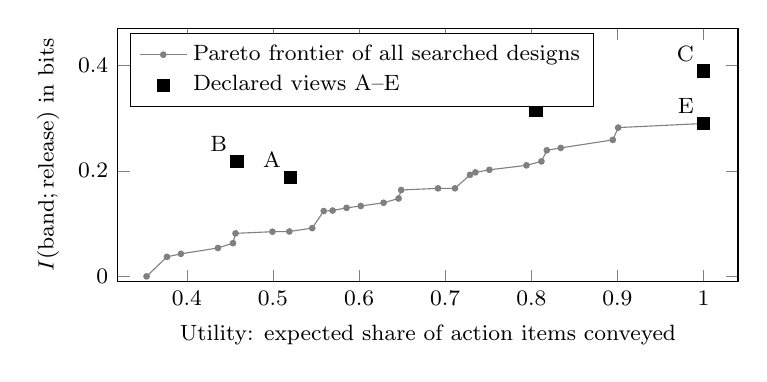
\begin{tikzpicture}
\begin{axis}[width=0.78\linewidth, height=4.8cm,
  xlabel={Utility: expected share of action items conveyed},
  ylabel={$I(\text{band}; \text{release})$ in bits},
  xmin=0.32, xmax=1.04, ymin=-0.01, ymax=0.47,
  tick label style={font=\footnotesize}, label style={font=\footnotesize},
  legend style={font=\footnotesize, at={(0.02,0.98)}, anchor=north west},
  legend cell align=left]
\addplot[gray, mark=*, mark size=1pt] coordinates {(0.3533,0.0000) (0.3770,0.0370) (0.3932,0.0427) (0.4362,0.0538) (0.4536,0.0629) (0.4566,0.0815) (0.4994,0.0846) (0.5191,0.0850) (0.5456,0.0914) (0.5590,0.1237) (0.5693,0.1247) (0.5855,0.1298) (0.6020,0.1333) (0.6285,0.1394) (0.6459,0.1475) (0.6489,0.1636) (0.6917,0.1667) (0.7114,0.1668) (0.7288,0.1923) (0.7351,0.1970) (0.7513,0.2018) (0.7943,0.2103) (0.8117,0.2178) (0.8180,0.2388) (0.8342,0.2433) (0.8946,0.2585) (0.9009,0.2818) (1.0000,0.2896)};
\addlegendentry{Pareto frontier of all searched designs}
\addplot[only marks, mark=square*, mark size=2.2pt, nodes near coords, point meta=explicit symbolic, every node near coord/.append style={font=\footnotesize, anchor=south east}] coordinates {(0.5205,0.1878) [A] (0.4582,0.2179) [B] (1.0000,0.3889) [C] (0.8054,0.3148) [D] (1.0000,0.2896) [E]};
\addlegendentry{Declared views A--E}
\end{axis}
\end{tikzpicture}
\caption{Leakage against utility, both exact for \code{main}. Grey: the designs that no other design beats on both axes, from the toolkit's exhaustive search over keeping, coarsening or dropping each field, plus task-output designs (Section~\ref{sec:toolkit}). Squares: the five declared views. D lies above and to the left of the frontier, so it is dominated; E (the checklist answers) is the frontier's full-utility end.}
\label{fig:tradeoff}
\end{figure}

Figure~\ref{fig:tradeoff} places the five views against the toolkit's exact frontier. Linking (C) gives full utility at the highest leakage. The declared coarsening D is dominated: the checklist answers E leak less (0.2896 against 0.3148 bits) and convey everything, and a field-level design that coarsens the share and the event, keeps the resolution, and drops the income pattern and the second payment flag reaches 0.8946 utility at 0.2585 bits. A and B leak less than any linked view but convey about half of the action items.

\subsection{Sensitivity to dependence and prevalence}
\label{sec:sensitivity}

\begin{table}[htbp]
\centering\footnotesize
\caption{Sensitivity scenarios. Exact columns are population values; the \code{nb} columns are test-split estimates with 95\% bootstrap intervals, and the log-loss difference is in bits. The baseline accuracy is 0.4000, except 0.3333 in \code{prev\_balanced} and 0.7000 in \code{prev\_skewed}.}
\label{tab:sensitivity}
\setlength{\tabcolsep}{3.5pt}
\begin{tabular}{@{}lcccccc@{}}
\toprule
& \multicolumn{2}{c}{Exact} & \multicolumn{3}{c}{\code{nb}, test split} \\
\cmidrule(lr){2-3}\cmidrule(l){4-6}
Scenario & C $-$ A & D $-$ C & C $-$ A & D $-$ C & D $-$ C log-loss \\
\midrule
\code{independence} & 0 & 0 & $-$0.0007 [$-$0.0080, 0.0077] & 0.0000 [$-$0.0090, 0.0090] & $-$0.0033 \\
\code{dep\_025} & +0.0128 & $-$0.0048 & $-$0.0010 [$-$0.0153, 0.0127] & $-$0.0013 [$-$0.0147, 0.0127] & +0.0015 \\
\code{dep\_050} & +0.0358 & $-$0.0137 & +0.0383 [0.0190, 0.0560] & $-$0.0227 [$-$0.0367, $-$0.0087] & +0.0125 \\
\code{dep\_075} & +0.0605 & $-$0.0214 & +0.0550 [0.0367, 0.0723] & $-$0.0223 [$-$0.0363, $-$0.0083] & +0.0339 \\
\code{main} & +0.0870 & $-$0.0287 & +0.0810 [0.0623, 0.0993] & $-$0.0183 [$-$0.0313, $-$0.0057] & +0.0465 \\
\code{prev\_balanced} & +0.0946 & $-$0.0292 & +0.0773 [0.0587, 0.0970] & $-$0.0240 [$-$0.0383, $-$0.0097] & +0.0456 \\
\code{prev\_skewed} & +0.0354 & $-$0.0174 & +0.0200 [0.0107, 0.0297] & +0.0010 [$-$0.0060, 0.0080] & +0.0237 \\
\bottomrule
\end{tabular}
\end{table}

The exact gains shrink as $\lambda$ falls, by construction (Table~\ref{tab:sensitivity}). The frozen S7 rule (\code{nb}'s point estimates of C $-$ A and C $-$ B non-decreasing over $\lambda = 0.25$ to 1) was met, but this is weak evidence: adjacent steps are within about two standard errors, the rule failed on the development split, and at $\lambda = 0.25$ \code{nb} realises no detectable gain ($-0.0010$ [$-0.0153$, 0.0127]) although the population gain is 0.0128. Effects of about one point are below this design's resolution.

Under skewed prevalence, H2a's direction fails on accuracy for \code{nb}: D $-$ C is +0.0010 [$-0.0060$, 0.0080], while log-loss still shows the loss (+0.0237 [0.0144, 0.0331] bits) and the exact gap is $-0.0174$. With a 0.7000 baseline, argmax accuracy is a poor leakage measure. For S8, in \code{prev\_skewed} \code{nb}'s accuracy in C, D and E is 0.7380, 0.7390 and 0.7247 but its macro recall is 0.4806, 0.4713 and 0.5054; in \code{prev\_balanced} the two agree (0.5743, 0.5503, 0.5460 against 0.5755, 0.5513, 0.5474).

\subsection{Controls}
\label{sec:controls}

\begin{table}[htbp]
\centering\footnotesize
\caption{\code{nb} accuracy on \code{main} by number of training labels (nested subsets of the training rows; exploratory, post-review). The 6,000-label row is the primary run; the last two rows are exact.}
\label{tab:learning}
\setlength{\tabcolsep}{5pt}
\begin{tabular}{@{}lccccccc@{}}
\toprule
Labels & A & B & C & D & E & C $-$ A & D $-$ C \\
\midrule
100 & 0.4440 & 0.5070 & 0.5050 & 0.5067 & 0.5153 & +0.0610 & +0.0017 \\
300 & 0.4667 & 0.5200 & 0.5397 & 0.5353 & 0.5443 & +0.0730 & $-$0.0043 \\
1,000 & 0.5140 & 0.5197 & 0.5783 & 0.5563 & 0.5563 & +0.0643 & $-$0.0220 \\
3,000 & 0.5187 & 0.5323 & 0.5963 & 0.5833 & 0.5633 & +0.0777 & $-$0.0130 \\
6,000 & 0.5193 & 0.5327 & 0.6003 & 0.5820 & 0.5663 & +0.0810 & $-$0.0183 \\
\midrule
\code{nb\_limit} & 0.5172 & 0.5271 & 0.5953 & 0.5755 & 0.5582 & +0.0782 & $-$0.0199 \\
Bayes ceiling & 0.5172 & 0.5271 & 0.6042 & 0.5755 & 0.5650 & +0.0870 & $-$0.0287 \\
\bottomrule
\end{tabular}
\end{table}

\paragraph{Pre-specified controls.} All passed. In \code{independence} the largest gap from the baseline was 0.0253 (\code{lookup} in A), within the 0.05 tolerance, which is wider than the effects of interest. In the positive control \code{nb} reached 1.0000 in A--D with 3,000 exposed test rows in each, and no other scenario had a direct exposure.

\paragraph{Exploratory controls (post-review).} With training labels permuted, no attacker beat the baseline in any view (the largest accuracy above the 0.3890 baseline was 0.0000). Attackers seeing only identifier characters and row position reached 0.3863 [0.3687, 0.4037]. In the learning curve (Table~\ref{tab:learning}), linking already helps an attacker with 100 labels (C $-$ A +0.0610) while the coarsening's effect is invisible there (D $-$ C +0.0017), and with few labels the checklist answers are about as useful to \code{nb} as the linked release (0.5443 against 0.5397 at 300 labels).

\subsection{Task outputs against coarsening (exploratory)}
\label{sec:evsd}

\begin{table}[htbp]
\centering\footnotesize
\caption{Exact values for variants of D and E in \code{main} (exploratory, post-review).}
\label{tab:variants}
\begin{tabular}{@{}lccc@{}}
\toprule
View & Bayes accuracy & MI (bits) & \code{nb\_limit} \\
\midrule
C (linked fine releases) & 0.6042 & 0.3889 & 0.5953 \\
D & 0.5755 & 0.3148 & 0.5755 \\
D without \code{income\_pattern} & 0.5667 & 0.2936 & 0.5667 \\
E & 0.5650 & 0.2896 & 0.5582 \\
E plus one item that needs \code{income\_pattern} & 0.5762 & 0.3110 & 0.5600 \\
E plus one item ``major expense settled in full'' & 0.5793 & 0.3252 & 0.5666 \\
E plus both & 0.5871 & 0.3456 & 0.5783 \\
E without \code{goal\_module} & 0.5380 & 0.2218 & 0.5305 \\
\bottomrule
\end{tabular}
\end{table}

The comparison of E with D was not pre-specified; it was raised after the test results were seen. Three statements are defensible.
\begin{itemize}
  \item \textbf{E always dominates the linked fine release,} by construction: same utility, and less leakage here (0.5650 against 0.6042).
  \item \textbf{E still leaks:} its ceiling is 0.1650 above the baseline, more than either single release (0.5172 for A, 0.5271 for B).
  \item \textbf{Against a coarsening, E is not ordered in general.} E's ceiling is below D's by 0.0105 (MI 0.2896 against 0.3148 bits), but one extra checklist item reverses this (Table~\ref{tab:variants}): an item needing the income pattern lifts E's ceiling above D's (0.5762 against 0.5755), though not its mutual information, and an item flagging a major expense settled in full lifts both (0.5793 and 0.3252 bits). D keeps \code{income\_pattern}, which the checklist never uses, while coarsening the fields the checklist needs: it is a task-unaware coarsening and an easy opponent.
\end{itemize}
The test split cannot resolve the E $-$ D gap: the sample oracle's E $-$ D accuracy is $-0.0010$ [$-0.0167$, 0.0143] on the primary run, and its interval excludes 0 in 1 of 6 seed runs (\code{nb}'s in 2 of 6). \code{nb} overstates the gap, because E's items share fields and naive Bayes is misspecified on E (unlimited-data accuracy 0.5582 against an exact 0.5650). Under skewed prevalence the exact gap shrinks to $-0.0024$. With the same schema, checklist and coarsening, E had lower Bayes accuracy than D in 88.5\% to 92.5\% of 400 random generators per setting (four settings, from mild perturbation to fully random tables) and lower mutual information in 90.0\% to 96.8\%: fairly robust to the probabilities, not to the checklist or the coarsening.

\section{A reusable release audit}
\label{sec:toolkit}

The pilot hard-codes one schema, generator, set of views and checklist, so we built \code{release\_audit}, a standard-library toolkit (\code{python3 -m release\_audit}) that asks the same questions of a user's own pipeline. It is not part of the pilot's inference.

\paragraph{Specification and evaluation.} A user writes one JSON file: the hidden target and its prior; fields assigned to stages, with exact conditional probability tables (a zero is a hard constraint); declared coarsenings; the task as checklist items given by ordered rules over raw fields; and the views to compare, including task outputs. When the raw space has at most 500,000 positive-probability records (a configurable limit), Bayes accuracy, mutual information, \code{nb\_limit}, exclusion masses and utility are exact. Above it the toolkit samples (by default 200,000 records), reports Bayes accuracy as a bracket between a held-out plug-in classifier (usually pessimistic) and resubstitution (optimistic), headlines the Miller--Madow corrected mutual information, and reports no exclusions, since a sampled zero is not a hard constraint (the v1.1.1 correction). Utility is by entailment: an item is conveyed if every positive-probability raw record yielding the released value gives it the same value. On the household specification this equals the pilot's strict renderer on all 328,320 record-view pairs, and the oracle's Bayes accuracies, mutual information and \code{nb\_limit} for A--E are reproduced.

\begin{table}[htbp]
\centering\footnotesize
\caption{The toolkit's per-field information budget for the household specification (\code{main}, exact, bits except the Bayes column). The reference is the full linked view: 0.3889 bits and Bayes accuracy 0.6042.}
\label{tab:budget}
\begin{tabular}{@{}lccccc@{}}
\toprule
Field & Stage & MI alone & MI lost if dropped & Bayes lost if dropped & MI lost by coarsening \\
\midrule
\code{r2.goal} & 2 & 0.0914 & 0.0587 & 0.0265 & \\
\code{r1.essential\_share} & 1 & 0.0865 & 0.0554 & 0.0254 & 0.0205 \\
\code{r1.payment\_flag} & 1 & 0.0850 & 0.0544 & 0.0229 & 0.0025 \\
\code{r2.payment\_flag} & 2 & 0.0846 & 0.0545 & 0.0224 & 0.0041 \\
\code{r2.resolution} & 2 & 0.0629 & 0.0697 & 0.0270 & 0.0412 \\
\code{r1.income\_pattern} & 1 & 0.0318 & 0.0192 & 0.0083 & \\
\code{r1.event\_code} & 1 & 0.0000 & 0.0281 & 0.0088 & 0.0281 \\
\code{r2.document\_status} & 2 & 0.0000 & 0.0000 & 0.0000 & \\
\code{r1.contact\_channel} & 1 & 0.0000 & 0.0000 & 0.0000 & \\
\bottomrule
\end{tabular}
\end{table}

\paragraph{Information budget and design search.} For each field the toolkit reports its information alone, the cost of dropping it from the full linked view and the cost of each declared coarsening (Table~\ref{tab:budget}), and it scans cross-stage pairs for synergy, $I(\text{target}; a, b) - I(\text{target}; a) - I(\text{target}; b)$, and for exclusions that appear only when stages are linked. On the household specification it finds the size-by-resolution interaction without being told where to look: \code{r1.event\_code} carries 0.0000 bits alone but costs 0.0281 bits when dropped, and the pair (\code{r1.event\_code}, \code{r2.resolution}) carries 0.1029 bits, a synergy of 0.0400, the largest of any pair, with the exclusion of \code{low} appearing only when the two are linked. The design search enumerates releases (keep, coarsen or drop each field, plus task outputs alone and with one field) and reports the frontier: for the household specification, 3,903 designs with 28 on the frontier (Figure~\ref{fig:tradeoff}); D is dominated.

\paragraph{Real-data mode.} From labelled records the toolkit estimates the same tables with cross-validated naive Bayes, a pairwise logistic regression that finds interactions unaided, learning curves and bias-corrected mutual information, without exclusions. On 400 records sampled from the grocery specification, plug-in resubstitution accuracy for the linked view is 0.9100 against an exact 0.8002.

\paragraph{A second example.} The grocery example is a different fictional pipeline: order, picking and delivery stages, a binary hidden attribute (young children in the household, prior 0.3000) and one invented cross-stage hard constraint (households without young children never ask for ``no bell'' on an afternoon slot). Linking the stages raises the exact ceiling from a 0.7000 baseline to 0.8002. Unaided, the budget finds the synergy between delivery window and doorstep instruction (0.0378 bits) and the exclusion it creates only when order and delivery are linked (mass 0.0330). The household ordering of E and D does not carry over: here the task outputs leak more than the declared coarsening (Bayes accuracy 0.7692 against 0.7190; 0.1843 against 0.1225 bits) while conveying every action item against 0.4667, and they keep the exclusion, because two items pass the window and the doorstep instruction through.

\paragraph{Release-design checklist.} The documentation condenses the pilot into seven lessons: a stable key across stages is the linkage; a verbatim pass-through leaks at full strength (dropping \code{goal\_module} from E lowers its information from 0.2896 to 0.2218 bits); cross-stage hard constraints give exclusions; default-filling renderers make unsupported claims; task outputs still leak; coarsen fields the task does not need first; check designs against the exact ceiling. A first specification of 8 to 12 fields is estimated at 3 to 6 hours; the toolkit has not been used outside this study.

\section{Limitations}

\textbf{Synthetic, no language model, linkage assumed.} Every probability is invented and no generator was validated against real households, so no result is a rate or effect size for real households or pipelines. No language model produces the findings, attacks them or renders the report, there is no free text, and nothing here says how language-model attackers or language-model-generated findings behave. Linkage is assumed, not tested.
\textbf{By construction.} The directions of H1 and H2a, H2b, S3, S6, ``E keeps full utility'' and ``E leaks no more than C'' follow from the design, and the attackers match the generator's structure, so their closeness to the ceilings says nothing about attackers in general.
\textbf{One coarsening, one checklist.} D is a single hand-picked, task-unaware coarsening, and the E-versus-D ordering reverses with one checklist item. Nothing here says that coarsening works or fails in general, or that minimal structured findings or task outputs are safe or unsafe as a class. Coarsening is not differential privacy~\cite{dwork2006calibrating}, which provably resists composition attacks~\cite{ganta2008composition}.
\textbf{Fragility and resolution.} H2a meets its criterion in 3 of 6 seed runs, and the power analysis used the wrong reference gap. Intervals cover test-sample uncertainty only, the independence tolerance (0.05) is wider than H2a or the E $-$ D gap, and a true gain of about one point (\code{dep\_025}) went undetected.
\textbf{Isolation, exposure, pre-specification.} Attacker isolation is process-level, not a sandbox, and the exposure scan finds fields named or valued as the band, not encodings of it. The freeze is self-attested, the first three commits fall within minutes, and the whole v1.0 study, from protocol to test results, was carried out in one evening, which bounds how much deliberation ``pre-specified'' implies; development results previewed the test outcome up to noise.
\textbf{Toolkit and literature.} Toolkit results are exact for the specification, not the world; synergy is scanned pairwise; the design search turns greedy beyond 5,000 field-option combinations; utility assumes the task is exactly the declared checklist. The prior-work search was not exhaustive.

\section{Conclusion}

In a small generator where every ceiling is computed exactly, linking two releases of structured findings raised a naive-Bayes attacker's accuracy by 6.8 to 8.1 points over a single release, and one cross-release pair ruled out a band outright, although neither release contained the band. A declared coarsening removed 2.9 points at the ceiling and 19.5\% of the action items and still leaked more than either single release; its confirmatory test passed on the pre-specified seed but in only 3 of 6 seed runs. The task's outputs kept full utility and still leaked; against a coarsening their ordering depended on the checklist. These illustrate established results, with sizes attached.

\section*{Code and data availability}

The git repository holds the protocol with its revision log, \code{FREEZE.json}, code, fixtures, summary results, the frozen v1.0 outputs, the toolkit with documentation, and this paper with \code{paper/NUMBERS.md} and \code{paper/check\_numbers.py}, which re-derive every number in the paper from the project's files. It is held locally at the time of writing; no DOI has been assigned yet. \code{python3 run\_pilot.py} regenerates every pilot output (the README gives about 95 s on a 12-core laptop), including the per-case files and datasets, which are too large for git and are regenerated byte for byte against SHA-256 hashes in \code{results/output\_manifest.json}; \code{--check-reproducible} runs the pipeline twice and compares every byte. The code uses only the Python standard library; all data are synthetic.

\section*{Acknowledgements and AI-assistance statement}

The code, analysis and manuscript were prepared with substantial assistance from Claude (Anthropic), an AI assistant, working under the author's direction. Separate AI agents carried out the literature search, the implementation and the independent senior review. The author is responsible for the content. The work used no paid API, cloud compute or external funding.

\begin{thebibliography}{99}\small
\setlength{\itemsep}{0pt}
\bibitem{ganta2008composition} S.~R.~Ganta, S.~P.~Kasiviswanathan, and A.~Smith. Composition attacks and auxiliary information in data privacy. In \emph{Proc.\ ACM SIGKDD (KDD)}, pp.~265--273, 2008. arXiv:0803.0032. \url{https://doi.org/10.1145/1401890.1401926}
\bibitem{taylor2026adaptive} S.~Taylor, P.~K.~Vippathalla, and J.~Coon. Adaptive privacy of sequential data releases under collusion. arXiv:2601.21859 [cs.IT], Jan.\ 2026 (v2 Jul.\ 2026). \url{https://arxiv.org/abs/2601.21859}
\bibitem{wang2006sequential} K.~Wang and B.~C.~M.~Fung. Anonymizing sequential releases. In \emph{Proc.\ ACM SIGKDD (KDD)}, pp.~414--423, 2006. \url{https://doi.org/10.1145/1150402.1150449}
\bibitem{xiao2007minvariance} X.~Xiao and Y.~Tao. M-invariance: Towards privacy preserving re-publication of dynamic datasets. In \emph{Proc.\ ACM SIGMOD}, pp.~689--700, 2007. \url{https://doi.org/10.1145/1247480.1247556}
\bibitem{brickell2008cost} J.~Brickell and V.~Shmatikov. The cost of privacy: Destruction of data-mining utility in anonymized data publishing. In \emph{Proc.\ ACM SIGKDD (KDD)}, pp.~70--78, 2008. \url{https://doi.org/10.1145/1401890.1401904}
\bibitem{samarati2001protecting} P.~Samarati. Protecting respondents' identities in microdata release. \emph{IEEE Trans.\ Knowledge and Data Engineering}, 13(6):1010--1027, 2001. \url{https://doi.org/10.1109/69.971193}
\bibitem{sweeney2002generalization} L.~Sweeney. Achieving $k$-anonymity privacy protection using generalization and suppression. \emph{Int.\ J.\ Uncertainty, Fuzziness and Knowledge-Based Systems}, 10(5):571--588, 2002. \url{https://doi.org/10.1142/S021848850200165X}
\bibitem{kifer2009definetti} D.~Kifer. Attacks on privacy and deFinetti's theorem. In \emph{Proc.\ ACM SIGMOD}, pp.~127--138, 2009. \url{https://doi.org/10.1145/1559845.1559861}
\bibitem{miklau2004formal} G.~Miklau and D.~Suciu. A formal analysis of information disclosure in data exchange. In \emph{Proc.\ ACM SIGMOD}, pp.~575--586, 2004. \url{https://doi.org/10.1145/1007568.1007633}
\bibitem{kawamoto2017compositionality} Y.~Kawamoto, K.~Chatzikokolakis, and C.~Palamidessi. On the compositionality of quantitative information flow. \emph{Logical Methods in Computer Science}, 13(3), 2017. arXiv:1611.00455. \url{https://doi.org/10.23638/LMCS-13(3:11)2017}
\bibitem{jayaraman2022imputation} B.~Jayaraman and D.~Evans. Are attribute inference attacks just imputation? In \emph{Proc.\ ACM CCS}, pp.~1569--1582, 2022. \url{https://doi.org/10.1145/3548606.3560663}
\bibitem{dwork2006calibrating} C.~Dwork, F.~McSherry, K.~Nissim, and A.~Smith. Calibrating noise to sensitivity in private data analysis. In \emph{Theory of Cryptography (TCC)}, LNCS, pp.~265--284, 2006. \url{https://doi.org/10.1007/11681878_14}
\bibitem{staab2024beyond} R.~Staab, M.~Vero, M.~Balunovi\'c, and M.~Vechev. Beyond memorization: Violating privacy via inference with large language models. In \emph{ICLR}, 2024. \url{https://arxiv.org/abs/2310.07298}
\bibitem{yukhymenko2024synthpai} H.~Yukhymenko, R.~Staab, M.~Vero, and M.~Vechev. A synthetic dataset for personal attribute inference. In \emph{NeurIPS Datasets and Benchmarks Track}, 2024. \url{https://arxiv.org/abs/2406.07217}
\bibitem{patil2025sum} V.~Patil, E.~Stengel-Eskin, and M.~Bansal. The sum leaks more than its parts: Compositional privacy risks and mitigations in multi-agent collaboration. arXiv:2509.14284, 2025. \url{https://arxiv.org/abs/2509.14284}
\bibitem{asif2026information} S.~Asif and M.~M.~Amiri. Information-theoretic privacy control for sequential multi-agent LLM systems. arXiv:2603.05520, 2026. \url{https://arxiv.org/abs/2603.05520}
\bibitem{zhou2025minimization} J.~Zhou, N.~Mireshghallah, and T.~Li. Operationalizing data minimization for privacy-preserving LLM prompting. arXiv:2510.03662, 2025. \url{https://arxiv.org/abs/2510.03662}
\bibitem{hu2026toolprivacybench} S.~Hu, L.~Liu, Z.~Meng, and Z.~Zhao. ToolPrivacyBench: Benchmarking purpose-bound privacy in tool-using LLM agents. arXiv:2606.28061, 2026. \url{https://arxiv.org/abs/2606.28061}
\bibitem{zharmagambetov2025agentdam} A.~Zharmagambetov, C.~Guo, I.~Evtimov, M.~Pavlova, R.~Salakhutdinov, and K.~Chaudhuri. AgentDAM: Privacy leakage evaluation for autonomous web agents. In \emph{NeurIPS Datasets and Benchmarks Track}, 2025. \url{https://arxiv.org/abs/2503.09780}
\bibitem{bagdasarian2024airgapagent} E.~Bagdasarian, R.~Yi, S.~Ghalebikesabi, P.~Kairouz, M.~Gruteser, S.~Oh, B.~Balle, and D.~Ramage. AirGapAgent: Protecting privacy-conscious conversational agents. In \emph{Proc.\ ACM CCS}, 2024. \url{https://arxiv.org/abs/2405.05175}
\end{thebibliography}

\end{document}
